\section{A WSN with Waspmotes: Background information}
\label{Chapter3}
\subsection{Introduction}
Waspmote is more than just hardware. It is an open source platform for wireless sensors, that especially focuses on low power consumption and autonomy. Battery lifetime greatly depends on the duty cycle and the used radio.\\ 
But it didn't just start with Waspmote and it will definitely not end with it. In 2007 developers from Libelium collaborated with the Arduino Team creating the first open hardware shield for Arduino, the "Arduino XBee Shield" \defcitealias{SHIELD}{Arduino Team, 2012}\citepalias{SHIELD}. The shield allowed an Arduino board to communicate wirelessly via ZigBee. Libelium used the shield to develop their first sensor device, the SquidBee, intended for creating sensor networks. Although the SquidBee is self-powered and implements wireless communications, it is more a sensor device than a wireless sensor device. It has a constant consumption of 50mA, discharging the battery within hours. The SquidBee was created for teaching and educational purposes only \defcitealias{SQUID}{Libelium, 2009}\citepalias{SQUID}. Since the platform was not radio certified the motes could not be deployed in real scenarios like cities, factories or even houses, so it did not fit Libelium's corporate customer requirements at all. However, the tone of an open hardware and open source wireless sensor device was definitely set.
\begin{figure*}[ht]
\centering
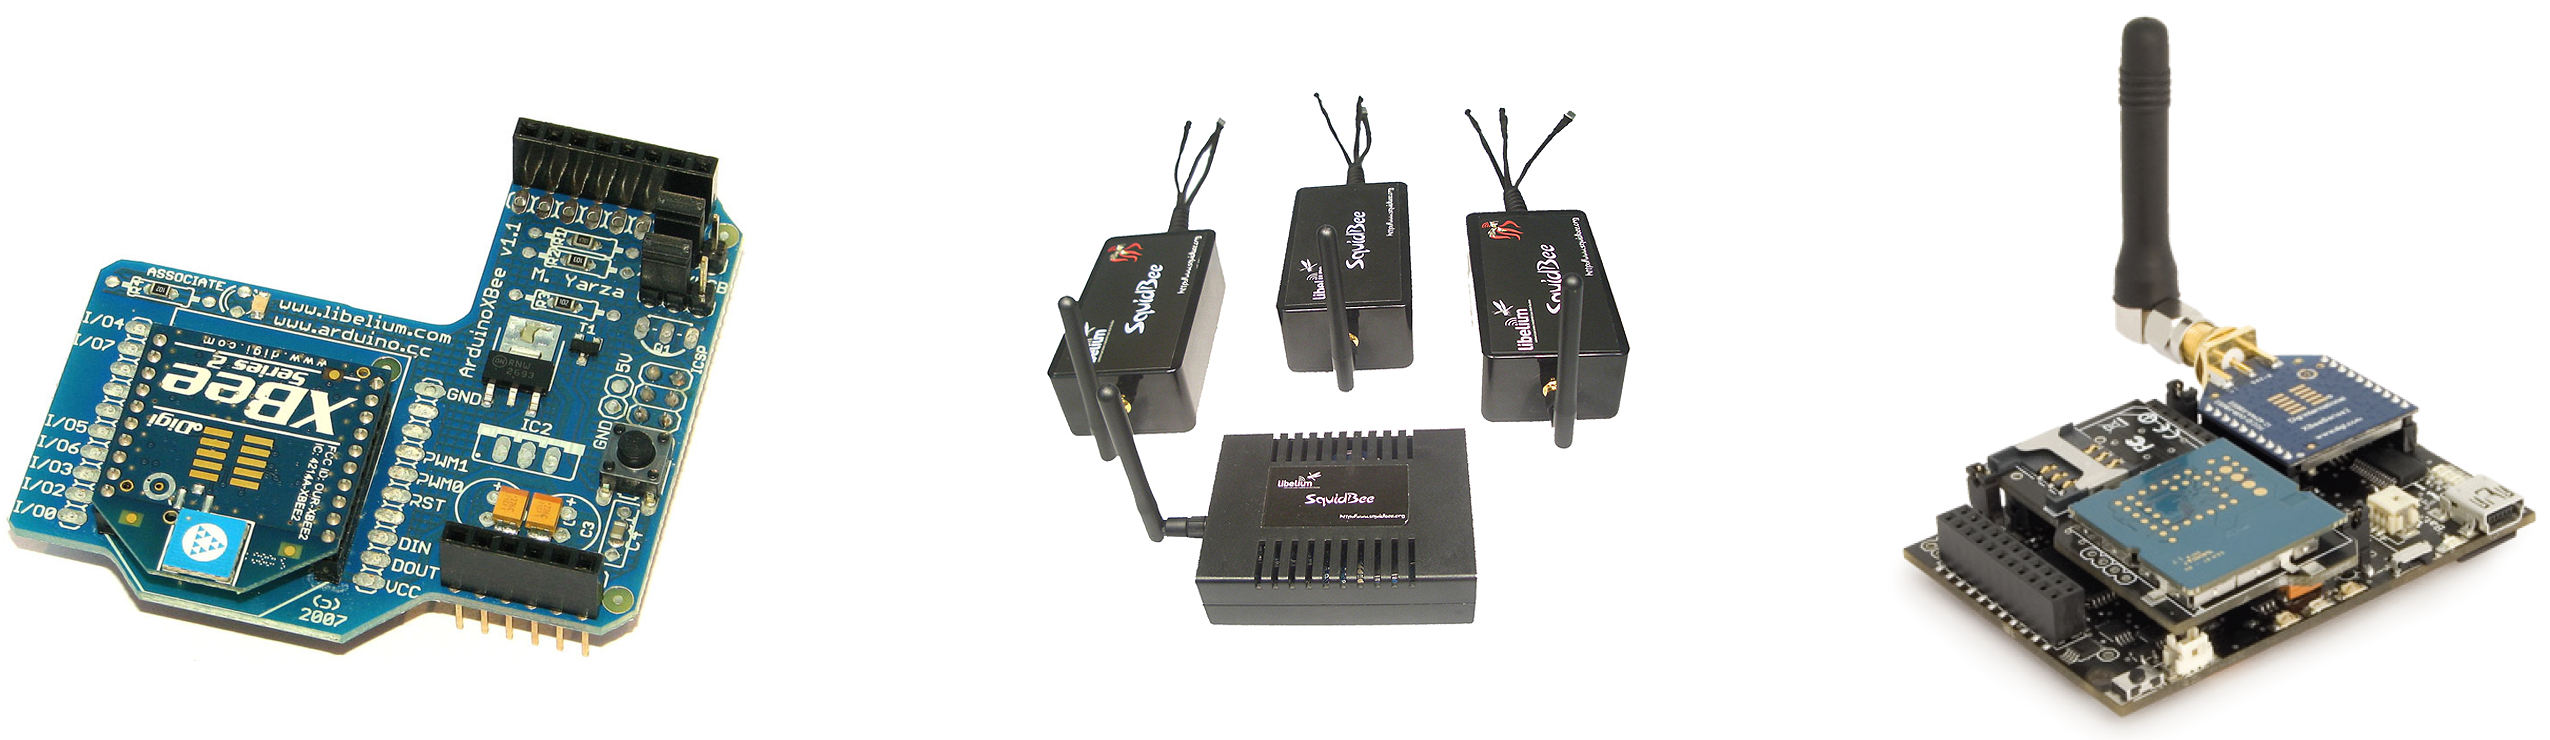
\includegraphics[width=0.95\textwidth]{chap3}
%\rule{30em}{0.5pt}
\caption{An Arduino XBee Shield (left), A Libelium SquidBee (middle) and a Libelium Waspmote V1.1 (right)}
\label{fig:chap3}
\end{figure*}\\
In 2009 the Waspmote (used for the WSN test-bed) was born, conform to all the above requirements and meeting three radio certification requirements\footnote{CE for Europe, FCC for the US and IC for Canada}. In addition the Waspmote was built with a complete modular philosophy. The idea behind this design is to integrate only the needed modules in each device, optimizing costs. This is why all modules are connected to the Waspmote via sockets\defcitealias{CH}{Cooking Hacks, 2013}\citepalias{CH}.\\Since its introduction, more than 2000 developers used Waspmote (v1.1) and the platform has received many suggestions and possible improvements. Libelium carefully listened to all these proposals and decided to bring out a new version with the name of Waspmote PRO (v1.2) in February 2013 \defcitealias{NEW}{WSN Research Group, 2013}\citepalias{NEW}. This new version comes with upgraded hardware and an improved API\footnote{Application Programming Interface (API)}, which is unfortunately not compatible with the older API. The most important improvements of the hardware is that the code can be uploaded much quicker and that the XBee radio must no longer be removed to do so. A new interrupt enables the XBee to wake the Waspmote PRO when XBee sleep modes are used \defcitealias{PRO}{Waspmote (v1.1) vs Waspmote PRO (v1.2), 2013}\citepalias{PRO}. To do this on the first version one must solder pin 13 of the XBee to the MUX\_RX pin of the Waspmote. This way interruptions caused by the XBee module can be captured, but all other interruption options (RTC\footnote{Real Time Clock (RTC)}, Accelerometer, etc.) will be masked by pin 13's output and will thus be lost.  The new version no longer has jumpers and there is no need for a coin battery. Regarding the API, Libelium claims it is much more robust and easier to use than the previous one. One big advantage of the new API is the support to send AT commands to the XBee.
%----------------------------------------------------------------------------------------
\subsection{Hardware}
\subsubsection{Modular Architecture}
As mentioned in the introduction, Waspmote is based on a modular architecture. Doing so optimizes costs and allows it to change according to the specific user's requirements. The available modules are split up into five categories: ZigBee, GSM - 3G/GPRS, GPS, Sensor Boards and Storage. Figure \ref{fig:waspMote1} indicates the Waspmote's main components.
\begin{figure}[ht]
\centering
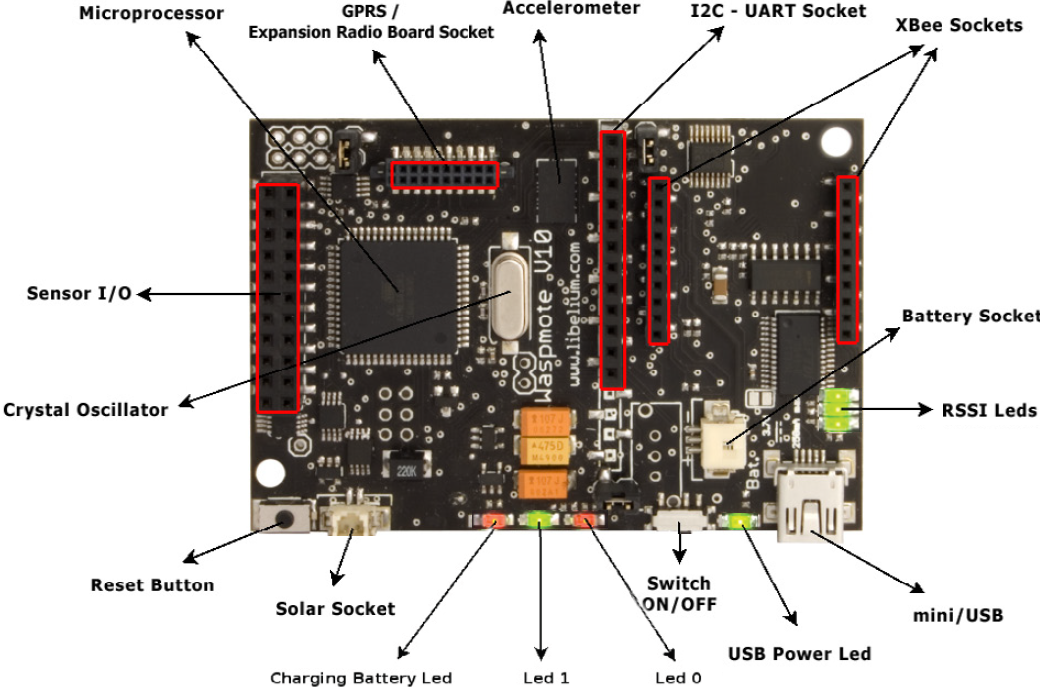
\includegraphics[width=0.46\textwidth]{waspmote2}
%\rule{30em}{0.5pt}
\caption{The main Waspmote components}
\label{fig:waspMote1}
\end{figure}
%-------------------------------------------
\subsubsection{XBee radio}
\label{ZBStructure}
The WSN nodes and the gateway make use of a XBee-ZB PRO radio. XBee is the brand name from Digi International for a family radio modules, based on the IEEE 802.15.4 standard \defcitealias{XBEE}{Digi International Inc, 2012}\citepalias{XBEE}. The PRO radio is a higher power, longer range version of the XBee-ZB radio.\\
To communicate with the XBee radio there are two modes: AT (transparent mode) and API (application programming interface). AT mode means that what you send to the XBee radio using RS232, the XBee radio will send to its default destination. Unless you send '+++', wait for the XBee to reply with OK, and then send an AT command. AT commands are used to change the configuration of the XBee radio. For instance the AT command OP requests the operating PAN ID. An AT command can also be used to change the default destination.\\
AT mode is fairly limited and only good for point to point communication since you can't really specify the destination unless you change the default destination all the time. So that is why the sensor network operates in API mode. This means that everything sent to the XBee radio, using serial communication, is now packetized.\\
API defines a number of different packets as can be found in chapter 9 of \defcitealias{XBEE}{XBee/XBee-Pro ZB RF Modules User Manual, 2012}\citepalias{XBEE}. An API packet is shown in figure \ref{fig:api}. It starts with \verb+0x7E+ as a start delimiter and is followed by the length of the data, excluding the checksum. Then an API-specific structure follows, which depends on the type of the packet.
\begin{figure}[t]%[htbp]
\centering
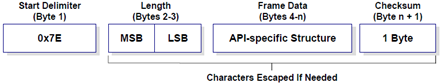
\includegraphics[width=0.48\textwidth]{api}
\caption{The UART Data Frame Structure}
\label{fig:api}
\end{figure} 
%\noindent
\begin{table}[t]%[!ht]
\begin{center}
\begin{tabular}[!ht]{|c|c|}
\hline
\textbf{API Frame Name} & \textbf{API ID}\\
\hline
AT Command & 0x08\\
\hline
ZigBee Transmit Request & 0x10\\
\hline
AT Command Response & 0x88\\
\hline
ZigBee Receive Packet & 0x90\\
\hline
\end{tabular}
\noindent
\caption{The API Frame Names and Values}
\label{tab:apis}
\noindent
\end{center}
\noindent
\end{table}
\label{api1}
\noindent
A reduced list of possible packets can be found in table \ref{tab:apis} (for the full list please see appendix \ref{AppendixF}). As mentioned, an AT command is used to alter the configurations of the ZigBee radio. This can of course also be done in API mode using the AT command packet.  The details about all the packets can be found in the datasheet. The only packet types used in this project are: 'ZigBee transmit request, \verb+0x10+' and “ZigBee receive packet, \verb+0x90+'. The reason only these packets are used is that Libelium puts its own structure inside the data of these packets. To send sample data not a 'ZigBee IO Data Sample Rx indicator' packet is sent but just a 'ZigBee transmit request, \verb+0x10+' packet, with the sample data as data. It's not the XBee radio that takes samples. It's the Waspmote's ATmega processor that samples the sensors and does some processing on them to go from a voltage to a more familiar value. Then this data has to be sent to the gateway and the only way to achieve this is by sending a data packet.\\
A ZigBee transmit request is shown in figure \ref{fig:api4}. This packet is used to send data from this ZigBee radio to a remote one. The remote ZigBee address is all that has to be known. These types of packets are constructed by the gateway to send out data to the Libelium nodes but also by Libelium nodes to send data to other Libelium nodes or to the gateway. Libelium has its own specific format for the RF Data as explained in section \ref{frames1} and as shown in figure \ref{fig:frames}. To reach the gateway, the address of the coordinator can be used, since the coordinator and gateway in our case are the same. This is convenient since the coordinator can always be addressed with \verb+0x0000000000000000+. The reason we chose the gateway as coordinator to be the same is that the coordinator receives a lot of traffic due to its role and the same goes for the gateway. So these two devices should be in the center of the network for efficiency reasons. Assigning one device for these two roles and trying to position this device as central as possible will ask for the least amount of routing overhead. However in this phase the position of the gateway is not optimal since it has to be stationed at module 14 for convenience. Module 14 is at the top of the building and packets coming from the ground floor will have to pass about two or three routers.\\
When data is received by a ZigBee radio, this radio will send out a ZigBee receive packet via its serial communication. An example of this packet can be found in figure \ref{fig:api5}. Again the received data has an additional format as specified in the Libelium Application header. 


%-------------------------------------------
\subsubsection{Microcontroller and memory}
\label{memory}
Because of the modular design of the Waspmote, the block diagram (see figure \ref{fig:block} \label{fig13}) is very simple. Waspmote integrates an 8-bit ATmega 1281 microcontroller with 128KB programmable flash, 8KB SRAM runtime memory and 4KB EEPROM memory. Since SRAM is built with cleverly combined MOSFETs it must not be periodically refreshed, but it is still volatile memory. The main advantage compared to DRAM is that, when moderately clocked like in the Waspmote, it consumes very little power.\\
The AVR\footnote{It is commonly accepted that AVR stands for Alf (Egil Bogen) and Vegard (Wollan)'s RISC processor, after its developers \citep{AVRWIKI}.} microcontroller was developed in 1996 by Atmel. It is a modified Harvard architecture 8-bit RISC\footnote{Reduced Instruction Set Computing (RISC)} microcontroller and was one of the first microcontroller families to implement flash memory for program storage (opposed to other microcontrollers at the time that were using 1-time programmable ROM, EPROM or EEPROM\footnote{(Electrically) (Erasable) (Programmable) Read-Only Memory (EEP)ROM}).\\
A Harvard computer architecture has separate storage and signal pathways for instructions and date. It can fetch instructions and data at the same time and can thus be faster than pure von Neuman architecture. Since most AVR instructions are 16 bit wide, the flash memory of the ATmega1281 with 128KB is organized as 64K x 16, so the Program Counter is 16 bits wide \defcitealias{ATMEGA}{Atmel ATmega 1281 Datasheet, 2012}\citepalias{ATMEGA}.\\
The architecture of the ATmega microcontroller modifies the Harvard architecture but the separate address space nature of a Harvard machine is preserved. In contrast to systems that add CPU cache, where data and instructions are unified, implementing the von Neumann model, the adaptation is much more subtle. The ATmega has an Extended Load Program (ELP) instruction which can allocate constant tables within the program memory address space (see figure \ref{fig:architecture} \label{fig14}). So the contents of the instruction memory can be accessed as data, saving scarce runtime memory. This however creates certain difficulties in programming, since the C Language was not designed for Harvard architectures (see section \ref{memory}). 
%-------------------------------------------
\subsubsection{Timers}
The Waspmote's system clock is an 8MHz quartz oscillator. This means that every 125 ns a machine language instruction is executed by the microcontroller. Keep in mind that one C++ instruction is several instructions in machine language.\\
To generate interrupts the Waspmote has an internal watchdog timer (WDT) and a Real Time Clock (RTC). The WDT is used to awake the Waspmote from \textit{Sleep} mode, because of its high precision. Thus, \textit{Sleep} mode allows small intervals, going from 16 milliseconds to a maximum of 8 seconds (see table \ref{tab:cons1}). To store an absolute time base the RTC can be used. Alarms programmed in the RTC specify days, hours, minutes and seconds. This clock is used to wake the Waspmote from \textit{Deep Sleep} or \textit{Hibernate}\footnote{It is important to notice that in \textit{Hibernate}, the RTC is no longer powerd through the main battery but through the auxiliary (button) battery. So when problems occur when using hibernate, it is recommended to measure the button battery's voltage and possibly it must be replaced.}, with intervals ranging from 8 seconds to even days.
%----------------------------------------------------------------------------------------
\subsection{Power considerations}
\label{pow}
\subsubsection{Waspmote power modes}
\label{dynPow}
The Waspmote has 4 operational modes: ON, Sleep, Deep Sleep and Hibernate. They differ in which type of interruptions they can be woken up and duration interval. Table \ref{tab:cons1} summarizes the Waspmotes operational modes. The main difference between the sleep modes and the hibernate mode is that, in a sleep mode the program is paused. Whereas with hibernate mode, all the Wasmpote's modules, including the microcontroller, are disconnected from the main battery. Only the RTC is powered through the auxiliary battery and can wake the node. This means the CPU is also switched of and does not remember any values from variables. When waking up the Waspmote reinitializes, the microprocessor is reset and the program restarts from the beginning. Both \textbf{setup} and \textbf{loop} routines are executed as if the main switch would be activated. By placing the \verb+ifHibernate()+ function in setup the program can determine if it came from a hardware reset or from a hibernate reset.\\
\begin{figure*}[!ht]
\centering
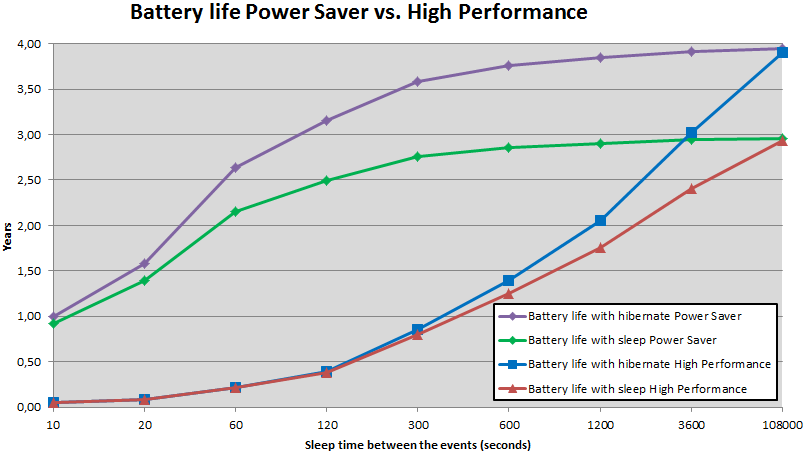
\includegraphics[width=0.74\textwidth]{battery2}
%\rule{30em}{0.5pt}
\caption{Battery life High Performance vs. Power Saver}
\label{fig:batCalcPSS}
\end{figure*}
%----------------------------------------------------------------------------------------
\subsubsection{Sampling sensors}
\label{duty}
To measure the sensors, we originally took 10 samples with 100 milliseconds recommended delay between the measurements. Since we want to make the energy consumption as low as possible we now do the iterations without delay. Appendix \ref{sensMeasuring} contains 60 test samples per sensor and indicates that there is no significant deviation on the average by removing this delay.\\ 
%-------------------------------------------
\subsubsection{Battery life estimation}
\label{batLife1}
In order to be able to provide recommended sensor measuring intervals this section will analyse the estimated battery life of the Waspmotes. Table \ref{tab:conss} enumerates the typical consumption of a node's common components.
\begin{table}[!ht]
\begin{center}
\begin{tabular}[!ht]{|c|c|}
\hline
\textbf{Action} & \textbf{Average Current}\\
\hline
Waspmote, ON & 9mA\\
\hline
Waspmote, sleep & 62$\mu$A\\
\hline
Waspmote, hibernate & 0,007$\mu$A\\
\hline
XBee, ON & 45mA\\
\hline
XBee, sending, & 105mA\\
\hline
Temperature & 6$\mu$A\\
\hline
Humidity & 380$\mu$A\\
\hline
CO$_{2}$ & 50mA\\
\hline
\end{tabular}
\caption{A Waspmote's typical power consumptions}
\label{tab:conss}
\end{center}
\end{table}
The batteries included with our Waspmotes are rechargeable Lithium-ion batteries with a capacity of 6600mAH. Lithium-ion has a self-discharge rate of typcially 1 to 2 percent per month \citep{LION} and since the batteries are new we expect high battery efficiency.\\
The application scenario for this battery test is as follows: the Waspmote will be turned on as short as possible and 4 sensors, namely temperature, humidity, pressure and battery level will be sampled. The node will take 10 samples for each sensor and calculate the average. Those values are put into one ZigBee packet and are sent to the gateway. By adapting the sleep time between the event we came to the rather disappointing results shown in figure \ref{fig:batCalcHP}. Please see appendix \ref{AppendixD} for more information.\\ 
Since the Waspmotes use this much energy when operating this way we will refer to it as the High Performance mode from now on. The next section calculates an alternative approach, referred to as the Power Saver mode. This nomenclature is continued in the program:
\usestyle{vs}
\includecode{pp.cpp}
%-------------------------------------------
\subsubsection{Battery life optimizations}
\label{powerSaver}
For end devices it is obviously recommended to turn on the XBee as little as possible, within a user defined limit.\\ Figure \ref{fig:batCalcPSS} shows the same results as the application scenario discussed in section \ref{batLife1} and adds the results for the Power Saver mode.\\
When the Power Saver mode is enabled, the Waspmote will awaken each time it has to sample data, but it will only send that data to the gateway once there are enough samples collected to send a maximum payload packet. Depending on whether one or two bytes are required per sample, 30 or 60 measurements can be taken before the Waspmote has to activate the XBee. In case the user requires a minimum responsiveness of the network there will also be an upper limit on the time a node may wait to send its collected samples.\\
As visible on figure \ref{fig:batCalcPSS}, \textit{Hibernate} has more influence in Power Saver mode, already extending battery life significantly at a 20 seconds interval compared to a 10 minutes interval in High Performance mode. Also the energy breakdown graph in figure \ref{fig:batCalcPS1} shows that the interval times must be increased much less before the dominant factor becomes self-discharge and sleep mode energy consumption, compared to figure \ref{fig:batCalcHP1}.\\
Finally, although Over the Air Programming (OTAP) is supported on Waspmotes, it should be limited to a minimum in order to obtain reasonable battery durations. Writing to FLASH takes about 83nAH per byte, whilst reading only takes about 1.1nAH per byte \citep{KTH}. 